\documentclass[11pt]{article}

% basic packages
\usepackage[margin=1in]{geometry}
\usepackage[pdftex]{graphicx}
\graphicspath{{./src/}}
\usepackage{amsmath,amssymb,amsthm}
\usepackage{custom}
\usepackage{lipsum}
\usepackage{booktabs}

\renewcommand\qedsymbol{$\blacksquare$}

% page formatting
\usepackage{fancyhdr}
\pagestyle{fancy}

\renewcommand{\sectionmark}[1]{\markright{\textsf{\arabic{section}. #1}}}
\renewcommand{\subsectionmark}[1]{}
\lhead{\textbf{\thepage} \ \ \nouppercase{\rightmark}}
\chead{}
\rhead{}
\lfoot{}
\cfoot{}
\rfoot{}
\setlength{\headheight}{14pt}

\linespread{1.03} % give a little extra room
\setlength{\parindent}{0pt} % reduce paragraph indent a bit
\setcounter{secnumdepth}{2} % no numbered subsubsections
\setcounter{tocdepth}{2} % no subsubsections in ToC

\begin{document}

% make title page
\thispagestyle{empty}
\bigskip \
\vspace{0.1cm}

\begin{center}
{\fontsize{30}{30} \selectfont \bf \sffamily ISSU0128 Mathematical Finance }\\
\vspace{24pt}
{\fontsize{14}{14} \selectfont \rmfamily Donald Kong} \\
\vspace{6pt}
{\fontsize{12}{12} \selectfont \ttfamily donk@donk.sg} \\
\vspace{24pt}
\end{center}

{\parindent0pt \baselineskip=15.5pt 
  \subsubsection{UCL Summer School Module Overview}
  This module provides a fundamental overview of mathematical finance. It
  begins with an overview of financial contracts, interest rates, and the value
  of money. Specifically, it discusses what constitutes a fair price for a
  contract and explains why fair prices are rarely used in everyday
  transactions. After that, we will investigate financial markets in a
  discrete-time setting, with the help of some revision on basic probability
  theory. The concept of risk-neutral asset pricing will be discussed with
  reference to pricing stocks and options in the exchange. The last part of the
  module introduces the fundamental concepts of stochastic calculus and
  concentrates on continuous time finance with the widely used Black-Scholes
  model. The goal of this course is to provide students with a broad
  understanding of the application to finance theory, while setting a solid
  theorical foundation to the field. This module is also useful for those who
  want to understand more about the field and related industries before fully
  committed to a Mathematical Finance pathway or a Mathematical Finance MSc, or
  simply a solid preparation to other undergraduate mathematical finance
  modules in general.
  \subsubsection{Suggested Textbooks and Readings}
  \begin{itemize}
    \item Baxter, Martin and Rennie, Andrew. Financial Calculus: An
      Introduction to Derivative Pricing. Cambridge University Press 1998
    \item Björk, Tomas. Arbitrage theory in continuous time. 3rd Edition, Oxford University Press 2009
    \item Garrett, S. J. An introduction to the mathematics of finance. Pearson Education India, 2006
    \item Hull, John C. Options, Futures and Other Derivatives. Elsevier/Butterworth Heinemann, 2013
    \item Ross, Sheldon. A First Course in Probability. Pearson, 8th Edition, 2008
    \item Shreve, Steven E. Stochastic calculus for finance. I. Springer-Verlags 2004
    \item Shreve, Steven E. Stochastic calculus for finance. II.\ Springer-Verlag 2004
  \end{itemize}
}

% make table of contents
% \newpage
\microtoc%
\newpage

% main content
\section{The Market, Value of Money, Securities and Strategies}
\subsection{Introduction}
\subsubsection{Terminologies}
\begin{definition}[Equity]
  The most basic of financial instruments is the \textbf{equity}, or known as the stock
  or the share.
\end{definition}
The \textbf{stockholder} (or \textbf{shareholder}) holds the right of
participating in the control of the company and receives \textbf{dividends}.
\begin{definition}[Dividend]
  \textbf{Dividends} are lump sum payments that are paid out every quarter or
  every six months to the stockholder, amount depending on the profitability of
  the company.
\end{definition}
\begin{definition}[Commodities]
  \textbf{Commodities} are raw products such as precious metals, oil and food products.
  Prices of commodities are unpredictable but tend to show seasonal effects,
  and are typically traded by people with no need for the material themselves.
\end{definition}

\subsection{Time Value of Money}
Depending on the market (in a deflating or inflating economy), but in general,
money today is has greater value than the same amount in a years time. This is
because money can be invested to ``produce'' more money, for instance through
interest payments.
\begin{remark}
  We consider investing money in a bank a \textbf{risk-free} investment and
  other financial instruments relative to this ``standard''.
\end{remark}
\begin{definition}[Effective Interest Rate]
  The interest rate associated with the basic time unit (typically defined $1$
  year) is the \textbf{effective interest rate} $r$.
\end{definition}
\begin{definition}[Nominal Interest Rate]
  When the frequency of compounding is not equal to the basic time unit, we call
  the associated interest rate the \textbf{nominal interest rate} $i$, defined:
  \[i=r\times \frac{t_{i}}{t_{r}}.\] 
  where $r$ is the effective interest rate, $t_{i}$ is the nominal interest
  time period, $t_{r}$ is the basic time unit of the effective interest rate.
\end{definition}
Suppose a nominal interest rate of $i$, with $m$ interest payments during a
year (once every $t=\frac{1}{m}$ years). The effective interest rate of each
sub-period $t$ years is $\frac{i}{m}$, and the effective interest rate for a
year is
\[r={(1+\frac{i}{m})}^{m}-1.\]
\subsubsection{Continuous Compounding}
As the interest payments happen at increasingly frequent intervals, $m\to\infty$:
\[\lim_{m \to \infty} {(1+\frac{r}{m})}^{m}= e^{r}.\]
\begin{proof}
  Using the binomial theorem,
  \begin{align*}
    {\left( 1+\frac{r}{m} \right)} ^{m}=&\sum_{i=0}^{m} \binom{m}{i}{\left( \frac{r}{m} \right)}^{i}\\
    =&1+\binom{m}{1}\frac{r}{m}+\binom{m}{2}{\left( \frac{r}{m} \right) }^{2}+\cdots+{\left( \frac{r}{m} \right)}^{m}\\
    =&1+r+\frac{m-1}{m}\frac{r^{2}}{2\mathpunct{!}}+\cdots+{\left( \frac{r}{m} \right) }^{m}
  \end{align*}
  Taking the limit $m\to\infty$:
  \[\lim_{m \to \infty} {(1+\frac{r}{m})}^{m}=1+r+\frac{r^{2}}{2\mathpunct{!}}+\frac{r^{3}}{3\mathpunct{!}}+\cdots= e^{r}.\]
  This is known as continuous compounding.
  \qed%
\end{proof}
\begin{remark}
  Continously compounded interest rates are used unless stated otherwise. The
  value of $b$ compounded over $T$ years at interest rate $r$ is: \[b\times
  e^{rT}.\]
\end{remark}
\subsubsection{Present Value}
\begin{definition}[Present Value]
  We define a mapping $P:\mathbb{R}\mapsto \mathbb{R}$ with initial condition
  $P(0)=k$ and interest rate $r$, such that:
  \[P(T)=ke^{rT}.\] 
  Due to the time value of money, cash flows in the future have smaller value
  that that in the present. We can then relate cash flows in the future (at
  time $T$) to their \textbf{present value} by:
  \[P(t)=P(T)e^{-r(T-t)},\quad t\in \left[ 0,T \right].\]
  This operation is known as \textbf{discounting}.
\end{definition}
\subsection{Fixed-Income Securities}
When a corporation wishes to borrow money from the public on a long-term basis,
it does so by issuing and selling debt securities known as \textbf{bonds}.
\begin{definition}[Bond]
  A \textbf{bond} is typically an interest-only loan, where interest is paid
  every period and principal is repaid at the end of the loan. It is defined by
  the \textit{face value/par value/nominal} (the lump sum), the
  \textit{coupons} and the \textit{maturity}.
\end{definition}
\begin{definition}[Coupons]
  The interest payments made on a bond is known as \textbf{coupons}. We can
  derive the \textit{coupon rate} from the \textit{annual coupon} $C$ and the
  face value $F$ of a bond $\frac{C}{F}$.
\end{definition}
The PV of a bond consists the PV of the face value and the annuity:
\begin{align*}
  PV_{\text{Bond}}=&PV_{\text{Face}}+PV_{\text{Coupon Cash Flow}}\\
  =&\frac{Face}{{(1+r)}^{t}}+\left(\frac{Annuity}{r}\right)\left( 1-\frac{1}{{(1+r)}^{t}} \right) 
\end{align*}
where $r$ is the interest rate, and $t$ the time to the bond's maturity.

\begin{definition}[Zero Coupon Bond]
  A \textbf{zero coupon bond} is a bond that pays no coupons at all. It must be
  offered at a price much lower than its face value.
\end{definition}

\subsection{Market Assumptions}
\begin{definition}[Arbitrage]
  Arbitrage refers to the possibility to make money without any risk.
\end{definition}
In a real market involving many participants, each motivated by making a
profit, any arbitrage opportunities that arises would vanish very quickly. We
make some market assumptions to ensure that there will only be a unique fair
price for a given bond.

\subsubsection{Terminologies}
\begin{definition}[Spot Price]
  We denote the price of any given stock or commodity at time $t\in
  \left.\left[0,\infty\right. \right)$ by $S(t)$. For present time (\textbf{spot time})
  $t=t_0$, $S(t_0)$ is the \textbf{spot price}.
\end{definition}
\begin{definition}[Price Process]
  For some $T\in \left( 0,\infty \right) $, the \textbf{price process} denoted ${\left(
  S(t) \right)}_{t\in [0,T]}=\left\{ S(t):t\in \left[ 0,T \right] \right\}$ for
  some function of randomness and time $S:\Omega\times \left[ 0,T
  \right]\mapsto [0,\infty)$. The price process is a random variable evolving
  through time, or a stochastic process.
\end{definition}
\begin{definition}[Underlyings]
  For contracts or derivatives written in relation to a certain amount of
  stocks or commodities, the particular stocks or commodities involved are
  referred to as the \textbf{underlyings}.
\end{definition}
\begin{definition}[Short-Selling]
  \textbf{Short-selling} involves selling an unowned or borrowed asset
  with the intention of buying it back later.
\end{definition}
\begin{definition}[Hedging]
  A strategy intended to reduce or minimise risk is known as \textbf{hedging}.
\end{definition}
\begin{definition}[Speculation]
  Taking a position in the market where the investor speculates that the price
  of the underlying asset will go up or down is known as \textbf{speculation}.
\end{definition}
\begin{definition}[Derivatives]
  \textbf{Derivatives} are financial contracts whose value depends from the
  values of some underlying asset(s).
\end{definition}

\subsubsection{Market Assumptions}
\begin{itemize}
  \item There are no transaction costs, e.g.\ no taxes, no bid-ask price, no
    brokerage fees. We call this market a \textbf{frictionless market}.
  \item The same risk-free rate of interest applies for borrowing and lending
    money (\textbf{market efficiency}) and the bank never goes bankrupt.
  \item There is an `absence' of arbitrage, as market participants take
    advantage of opportunities as they occur.
  \item It is always possible to buy/sell something in any amount at its fair
    price.
\end{itemize}

\subsection{Forward Contract}
\begin{definition}[Forward Contracts]
  \textbf{Forward Contracts} are agreements between two parties to buy or sell
  an asset $S(T)$ at a specified future time $T$ at a specified delivery price
  $K$, known as the maturity or delivery date.  Participants are obligated to
  buy or sell the asset at maturity.
\end{definition}
One of the parties assumes a long position to purchase the underlying asset at
time $T$, and the other party assumes a short position to sell the underlying
asset.
\subsubsection{Pay-off}
Pay-off per unit of asset from the long position in a forward contract: $S(T)-K$.\\
Pay-off per unit of asset from the short position in a forward contract: $K-S(T)$.
\begin{figure}[h!]
  \centering
  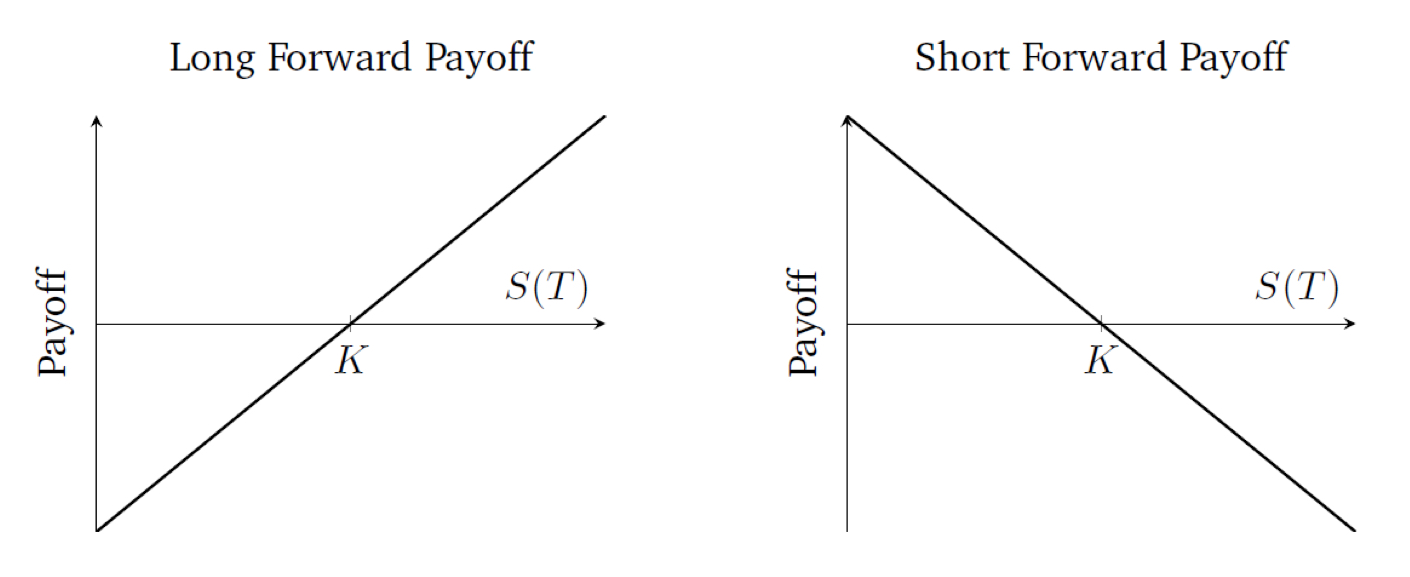
\includegraphics[width=0.8\textwidth]{forward-payoff}
\end{figure}\\

\centering
\begin{tabular}{c c c}
\toprule
Holding & Value at time $t$ & Value at maturity $T$\\
\midrule
Forward & $+0$ & $S(T)-K$\\
Stock & $-S(t)$ & $-S(T)$\\
Bank & $+S(T)$ & $S(t)e^{r(T-t)}$\\
\midrule
Total & $0$ & $S(t)e^{r(T-t)}-K$\\
\bottomrule
\end{tabular}

\raggedright%
\begin{prop}[Fair Delivery Price of a Forward Contract]
  The arbitrage free delivery price of a forward contract is a map $K: \left[
  0,T \right]\times [0,\infty)\mapsto [0, \infty)$ such that:
  \[K(t,T)=S(t)e^{r(T-t)}.\] 
\end{prop}
\begin{prop}[Convergence to Spot Price]
  The fair no-arbitrage delivery price of a forward contract converges to the spot price
  of the underlying asset as we approach maturity. That is,
  \[\lim_{t \to T} K(t,T)=S(T).\]
\end{prop}

\subsection{Options Contracts}
Options are similar to forward contracts, but without their obligatory aspect.
Additionally, options are sold for a certain specified initial amount, known as
the \textit{premium}.  The holder of a option has the decision whether to
execute the contract or not.  There are two types of options contracts:
\begin{itemize}
  \item A \textbf{call option} gives the holder the right to buy the underlying
    asset $S$ at a certain future \textit{expiration date} $T$ for a certain
    \textit{strike price} $K$.
  \item A \textbf{put option} gives the holder the right to sell the underlying
    asset $S$ at a certain future \textit{expiration date} $T$ for a certain
    \textit{strike price} $K$.
\end{itemize}
\begin{remark}
  There are two subtypes of the options contracts:
  \begin{itemize}
    \item \textbf{European options} can be exercised only on the expiration date itself.
    \item \textbf{American options} can be exercised at any time up to the expiration date.
  \end{itemize}
  Due to the additionally flexibility, premiums of the same parameters will be
  higher in American options than European options.
\end{remark}
\subsubsection{Pay-off}
Suppose an investor purchases a European call option on a certain stock with a
strike price $K=10$ and an expiration datae in three months.
At maturity, there are two possibilities for $S(T)$:
 \begin{enumerate}
  \item $S(T)<K$:
    The investor will choose not to exercise the option, as they can purchase
    the stock in the market for a better price. There is no profit to be made
    from the option and the investor loses money by paying for the premium.
  \item $S(T)>K$:
    The investor will exercise the option and will make a profit by selling them
    immediately at the spot price.
\end{enumerate} 
\begin{figure}[h!]
  \centering
  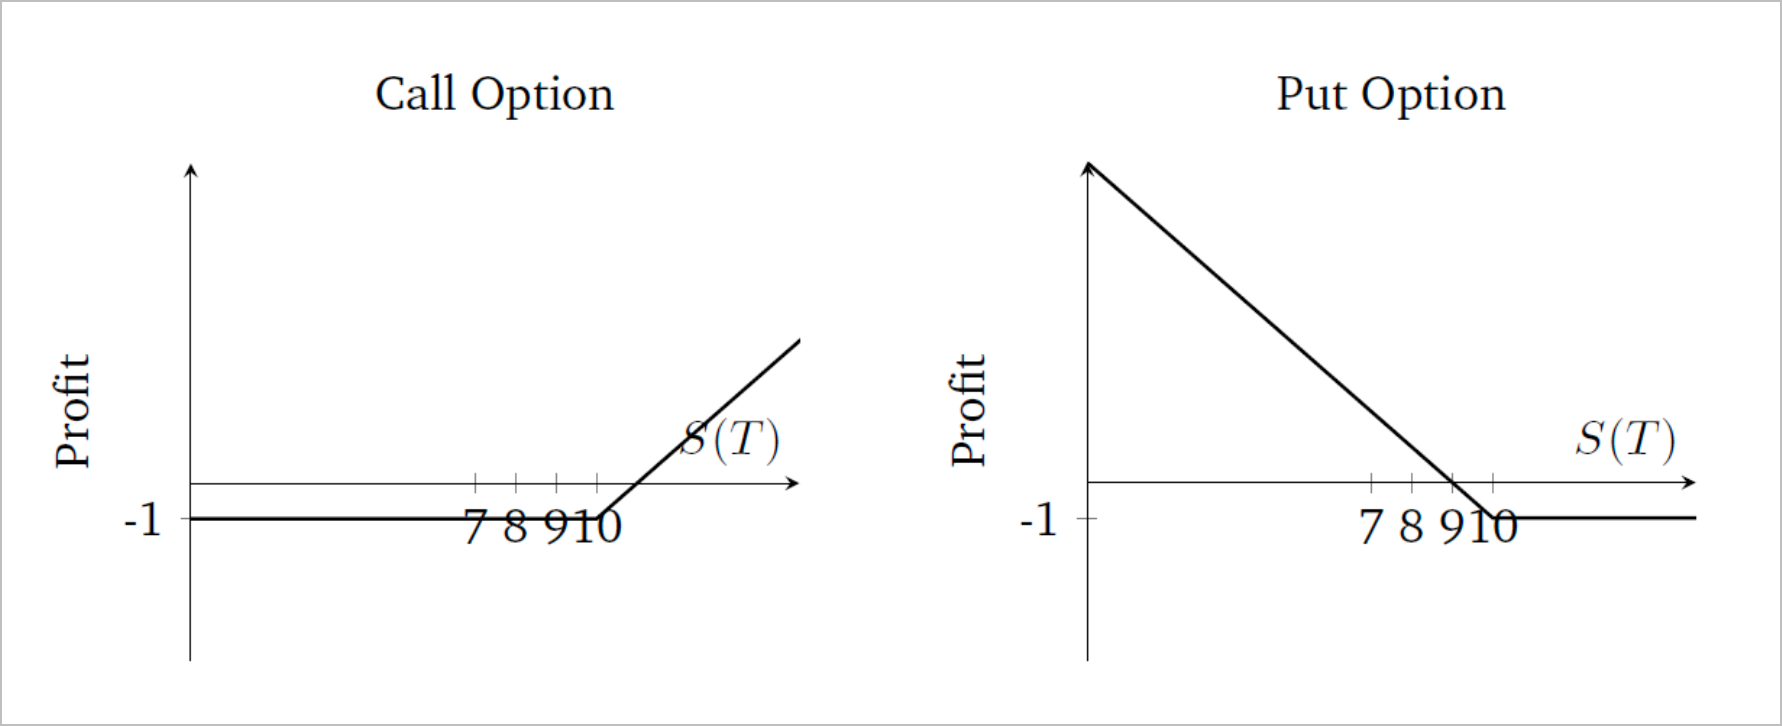
\includegraphics[width=0.8\textwidth]{option-long-payoff}
\end{figure}
The pay-off of the long European call is given by $\max \left\{ S(T)-K,0
\right\}$ and we define the \textbf{call function} the map
$f:\mathbb{R}\mapsto \mathbb{R}$:
\[f(x)=\max \left\{ x-K,0 \right\}={(x-K)}^{+}.\]
Similarly, the pay-off of the long European put is given by $\max \left\{
K-S(T),0 \right\}$ and we define the \textbf{put function} the map
$f:\mathbb{R}\mapsto \mathbb{R}$:
\[f(x)=\max \left\{ K-x,0 \right\}={(K-x)}^{+}.\]

\centering
\begin{tabular}{c c c}
  \toprule
  Contract & Position & Pay-off \\
  \midrule
  Call & Long & $\max \left\{ S(T)-K,0 \right\}$ \\
  Call & Short & $-\max \left\{ S(T)-K,0 \right\}$\\
  \midrule
  Put & Long & $\max \left\{ K-S(T) \right\}$\\
  Put & Short & $-\max \left\{ K-S(T),0 \right\}$ \\
  \bottomrule
\end{tabular}

\raggedright

\subsubsection{Replicating Portfolio}
\begin{definition}[Replicating Portfolios]
  We say that a portfolio is \textbf{replicating} with relation to a given
  contract if at maturity time, the future value of the replciating portfolio
  is the same as the future value of the contract.
\end{definition}
\begin{theorem}[Law of One Price]
  In an arbitrage free market, two portfolios with identical future values must
  have identical present values.
\end{theorem}
We see that replicating portfolios (by definition) have the same value at the
present and in the future.

\subsubsection{Put-Call Parity}
\begin{theorem}[Put-Call Parity]
  Consider a call and put option written on a stock $S$ with maturity $T$ and
  strike price $K$. Let ${\left( c_t \right)}_{t\in \left[ 0,T \right]}$ and
  ${\left( p_t \right)}_{t\in \left[ 0,T \right]}$ denote the fair prices of a
  call and put option at time  $t\in \left[ 0,T \right]$. Then for any $t\in \left[ 0,T \right]$,
  \[c_{t}+Ke^{-r(T-t)}=p_{t}+S(t).\] 
\end{theorem}
\begin{proof}
  Consider two portfolios:\\
  \textit{Portfolio A}: A cash amount of £$Ke^{-rT}$ and a European call option
  written on a non-dividend-paying stock.\\
  \textit{Portfolio B}: A European put option written on a non-dividend-paying
  stock and one share.
  At time $t=T$, we have:
  \[V_A=\max \left\{ S(T),K \right\}\qquad V_B=\max \left\{ S(T),K \right\}.\]
  They are replicating portfolios and by the law of one price, the values
  of the portfolios at time $t=0$ should be equal. That is:
  \[c_{0}+Ke^{-rT}=p_{0}+S(0).\]
  We obtain the put-call parity at time $t=0$ which applies $\forall t\in [0,T]$ by finding the
  values of the portfolios at time $t$.
  \qed%
\end{proof}

\subsubsection{Synthetic Securities}
Using the put-call parity, we may create synthetic versions of other
securities, of which replicates or simulate a security by combining the
features of other assets.
\begin{example}[Synthetic Stock]
  A long position in a underlying stock is equivalent to a long position in a
  call option, a long position in a risk-free bond and a short position in a
  put option.
  \[S(0)=c_0+Ke^{-rT}-p_0.\] 
\end{example}
\begin{example}[Synthetic Put Option]
  A long position in a put option is equivalent to a long position in a call
  option, a long position in a risk-free bond and a short position in the
  underlying stock.
  \[p_0=c_0+Ke^{-rT}-S(0).\] 
\end{example}

\subsection{Trading Strategies}
With these financial objects, we may derive further common strategies driven by
speculation motives or desires to hedge, of which can
\begin{enumerate}
  \item involve a single option and a stock
  \item involve two or more options of the same type (\textbf{spreads})
  \item involve both calls and puts on the same stock (\textbf{combinations})
\end{enumerate}
\begin{remark}
  We ignore the time value of money in calculating the profit functions, that
  is, $r=0$. Profits are calculated simply by subtracting the initial cost from
  the final payoff.
\end{remark}
\subsubsection{Covered Calls, Protective Puts}
These strategies seek to reduce the risk from the short position of a call
option, or the risk of a sharp decrease in the value of a stock. We hedge the
unlimited/large downside risk of large price changes, by holding a long
position in the underlying stock, or the long position in a put option.
\begin{figure}[h!]
  \centering
  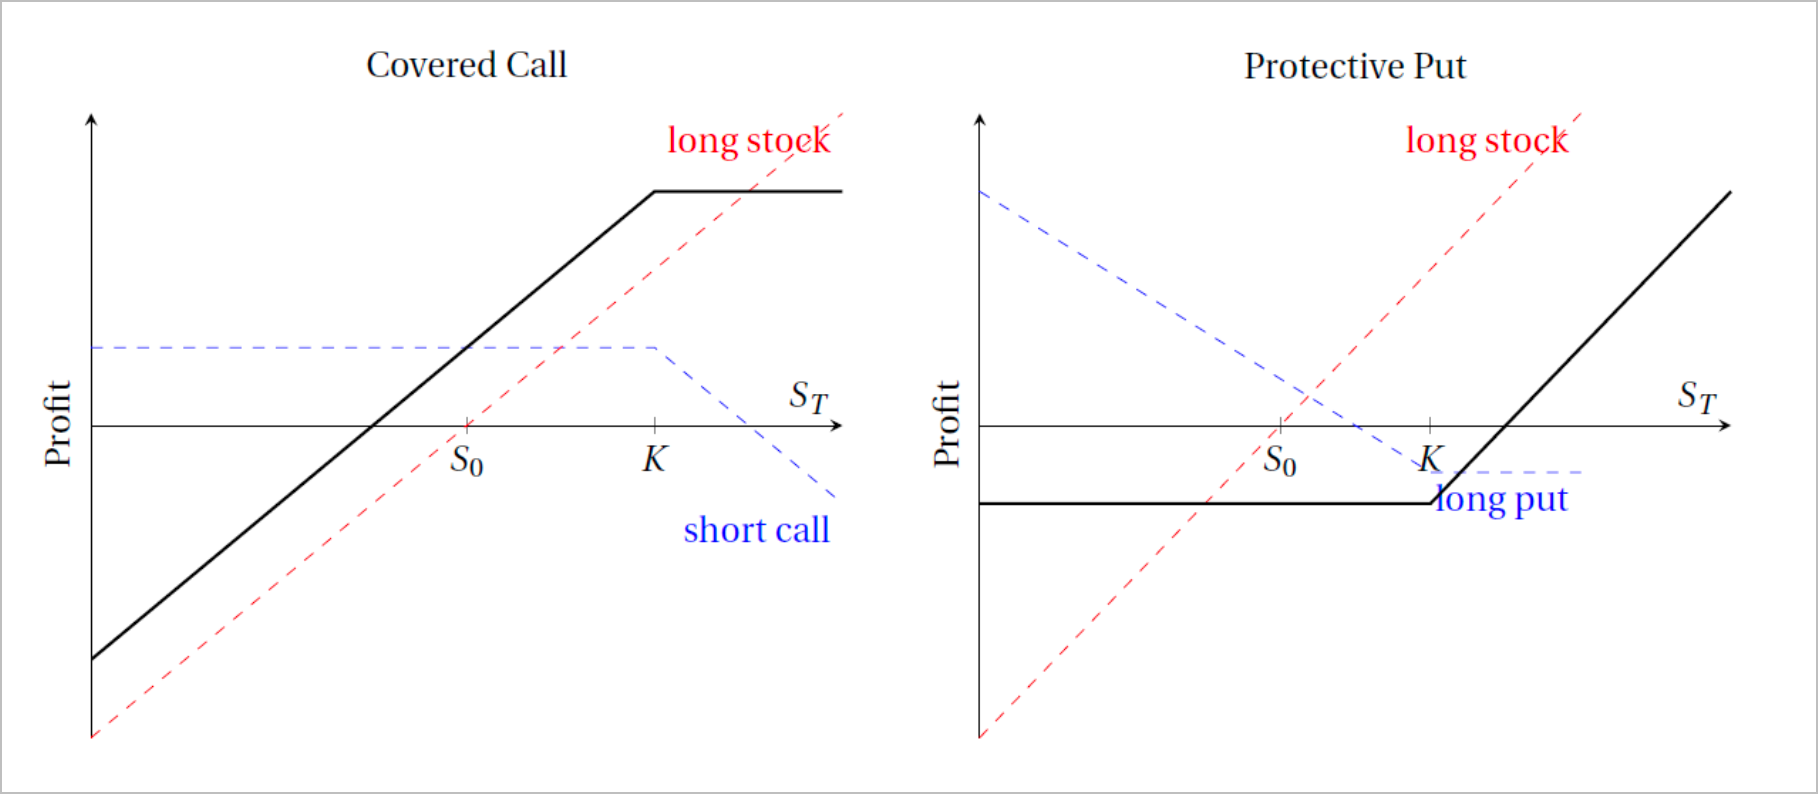
\includegraphics[width=0.8\textwidth]{covered-protective}
\end{figure}
An investor may also short these financial objects, of which the profit
diagrams is the negative of those above.
\subsubsection{Spreads}
A spread is a portfolio consisting two or more options of the same type, with
different positions.
\begin{itemize}
  \item \textbf{Bull Spread}: long one call with strike price $K_l$, and short
    one call with higher strike price $K_s>K_l$ 
  \item \textbf{Bear Spread}: long one call with strike price $K_l$, and short
    one call with lower strike price $K_s<K_l$ 
  \item \textbf{Butterfly Spread}: long two calls with strike prices
    $K_{l1},K_{l2}$ and short two calls with strike price $K_s = \frac{K_{l1} +
    K_{l2}}{2}$
\end{itemize}
\subsubsection{Combinations}
A combination is a portfolio consisting both call and put options with the same
position on the same stock. The strikes and maturities of all the options
included are the same.
\begin{itemize}
  \item \textbf{Straddle}: long one call and one put
  \item \textbf{Strips}: long one call and two puts
  \item \textbf{Straps}: long one put and two calls
  \item \textbf{Strangles}: long a put and a call
\end{itemize}

\section{Risk Neutral Asset Pricing}
\subsection{The One-Period Model}
\subsubsection{Introduction and Setup}
The market consists of a stock and a bank account over a single period $n\in
\left\{ 0,1 \right\}$. The bank account pays interests discretely at a rate
$r$. The stock price is a stochastic process ${\left( S_{n} \right)}_{n=0,1}$,
where $S_0\in \mathbb{R}^{+}_{*}$ and $S_1$ is a Bernoulli random variable such that:
\[S_1=S_0Z\quad\text{ where }\quad Z:\Omega \mapsto \left\{ u,d \right\},P[Z=u]=p_u, P[Z=d]=p_d.\]
For positive constants $d,u,p_u,p_d$, such that $d<u$, we refer to the market
model as the one-period binomial model.
\begin{definition}[Trading Strategy]
  We refer to a vector $h:=\left( x_0,y_0 \right)\in \mathbb{R}^{2}$ as
  the \textbf{portfolio} or \textbf{trading strategy}, where $x_0$ denotes the
  number of units of money in the bank account and $y_0$ denotes the
  number of units of stocks at time $t=0$ or period $n=0$.
\end{definition}
\begin{definition}[Value Process]
  We define the \textbf{value process} of a portfolio $h$ to be
  \[V_{n}^{h}:=x_0B_{n}+y_0S_{n},\qquad n=0,1.\]
\end{definition}
\begin{definition}[Arbitrage]
  A portfolio $h$ in the one-period binomial model is an \textbf{arbitrage portfolio} if the following
  conditions hold:
  \begin{itemize}
    \item $V_0^{h}=0$ 
    \item $P[V_1^{h}\ge 0]=1$
    \item $P[V_1^{h}> 0]>0$
  \end{itemize}
  That is, we are guaranteed a nonzero profit without risk.
\end{definition}
If no such portfolio exists, we say that the market is \textit{free of arbitrage}.
\begin{prop}[Free of Arbitrage]
  The one-period binomial model is free of arbitrage if and only if
  \[d\le 1+r\le u.\]
\end{prop}
\subsubsection{Risk-Neutral Measure}
With a market free of arbitrage in the one-period binomial model, we have $d\le 1+r\le u$ and
\[\exists q_u,q_d\in [0,1]\qquad \text{s.t.}\qquad 1+r=q_u\cdot u+q_d\cdot d\quad \text{and}\quad q_u+q_d=1.\] 
These conditions have the unique solution:
\[q_u=\frac{(1+r)-d}{u-d}\qquad\text{and}\qquad q_d=\frac{u-(1+r)}{u-d}.\]
We interpret $q_u$ and $q_d$ as a new probability measure $\mathbb{Q}$ where
the $\mathbb{Q}[Z=u]=q_u$ and $\mathbb{Q}[Z=d]=q_d$, of which the expected
value of the value of the stock is equal to that of the riskless bank account.
It follows that the value of the stock today is the discounted expected value
of the stock in the future.
This $\mathbb{Q}$ is known as the \textbf{risk-neutral measure}, (or
\textbf{martingale measure}), as we are indifferent between the bank account or
the stock under this measure. 
\begin{prop}[Existence of Risk-Neutral Measure]
  There exists such a measure if and only if the model is arbitrage free.
\end{prop}
\subsubsection{Contingent Claims}
With this market model, we are able to introduce derivative products and find the
fair prices for such objects.
\begin{definition}[Contingent Claim]
  A \textbf{contingent claim} is a stochastic variable $X$ of the form
  $X=\Phi(S_1)$ where $S_1$ is the stochastic variable representing the value
  of the stock.
\end{definition}
The real valued function $\Phi$ is known as the contract function.
\begin{notation}[Price Process of a Claim]
  We denote $\Pi\left( n;\Phi\left( S_1 \right)  \right) $ the price operator
  associated with the claim which returns the price of the claim at period $n$.
\end{notation}
\begin{definition}[Reachability of a Claim]
  We say that a contingent claim $X$ is \textbf{reachable} if there exits a portfolio
  $h$ such that
  \[P(V_1^{h}=X)=1.\]
  $h$ is known as the \textit{hedging portfolio} or a \textit{replicating
  portfolio}.
\end{definition}
By the law of one price, the hedging portfolio has the same value as the contingent claim:
\[\Pi\left( n;\Phi \right) =V_{n}^{h}.\]
By solving the equation at $n=1$ in the one-period binomial model,
\[V_1^{h}=\Phi=\Pi\left( 1;\Phi \right) \iff
  \begin{cases}x(1+r)+yS_0u=\Phi(S_0u)&Z=u\\x(1+r)+yS_0d=\Phi(S_0d)&Z=d\end{cases}\] 
which has a solution due to the no arbitrage condition $d<u$, $h^{*}=\left( x^{*},y^{*} \right) $ where:
\begin{align*}
  x^{*}=&\frac{1}{1+r}\frac{u\Phi\left( S_0d \right) -d\Phi\left( S_0u \right) }{u-d}\\
  y^{*}=&\frac{1}{S_0}\frac{\Phi\left( S_0u \right) -\Phi\left( S_0d \right) }{u-d}
\end{align*}
We have the price of the claim:
\[\Pi\left( 0;\Phi \right)=\frac{1}{1+r}E_{\mathbb{Q}}\left[  \Phi\left( S_1(Z) \right) \right].\] 
\begin{theorem}[Fair Price of a Contingent Claim]
  If the binomial model is free of arbitrage, then any claim $\Phi$ is replicable and
  the no-arbitrage price of $\Phi$ is given by
  \[\Pi\left( 0;\Phi \right)=\frac{1}{1+r}E_{\mathbb{Q}}\left[  \Phi\left( S_1\right) \right].\]
  where $\mathbb{Q}$ is the risk-neutral probability measure.
\end{theorem}
\begin{remark}
  The continuously compounded version of the one-period binomial measure
  follows, where $(1+r)$ is replaced by the continuously compounded interest
  $e^{rt}$
\end{remark}
\subsubsection{Risk-Free Portfolio Pricing}
We may also derive a portfolio such that there is no risk of the value of the
portfolio at its maturity. The value of the portfolio is independent of the
value of the underlying asset.\\
We find such a portfolio by solving for a portfolio $h=(0,\triangle)$ with a
short position in a European call with contract function $\Phi$ such that:
\[\triangle\cdot S_1(u)-\Phi(S_1(u))=\triangle\cdot S_1(d)-\Phi(S_1(d)).\]
\begin{remark}
  A riskless portfolio pays the exact same as a deposit in the bank account.
\end{remark}

\subsection{Multi-Period Model}
We extend the one-period binomial model into a multi-period binomial model, a
discrete-time model with $N \in \mathbb{N}$ periods and a running time index
$n=0,\ldots,N$. The time periods have a fixed time length $\triangle t$ and the
total time of the $N$ periods is $T=N\triangle t$.
\subsubsection{Setup}
The two underlying assets, namely a bond with price process
${(B_{n})}_{n=0,\ldots,N}$ and a stock with price process
${(S_{n})}_{n=0,\ldots,N}$, are defined as follows:
\[\text{Bank/Bond}=\begin{cases}B_0=1\\B_{n+1}=(1+r)B_{n}={(1+r)}^{n+1}\end{cases}\] 
\[\text{Bank/Bond}=\begin{cases}S_0=1\\S_{n+1}=S_{n}Z_{n}\end{cases}\] 
where we have a collection of i.i.d.\ Bernoulli r.v. $Z_0,\ldots,Z_{N-1}$.
\begin{definition}[Portfolio Strategy]
  We extend the portfolio strategy to a stochastic process
  \[\left\{ h_{n}=(x_{n},y_{n}) : n=1,\ldots,N\right\}.\]
  where each $h_{n}$ is a function of the stock prices. $h_0=h_1$ by
  convention. The corresponding \textit{value/wealth process} is
  \[V_{n}^{h}=x_{n}B_{n}+y_{n}S_{n}=x_{n}{(1+r)}^{n}+y_{n}S_{n}.\]
\end{definition}
\begin{definition}[Self-Financing Strategy]
  We say a portfolio strategy $h_{n}$ is a \textbf{self-financing strategy} if
  \[x_{n}(1+r)+y_{n}S_{n}=x_{n+1}(1+r)+y_{n+1}S_{n}.\]
  There is no extra capital into the portfolio at any time. We assume all
  portfolio strategies are self-financing.
\end{definition}
\begin{theorem}[Arbitrage-Free Market Model]
  For some $d<u$, the model is arbitrage-free if and only if $d\le 1+r\le u$,
  and there exists a unique risk-neutral measure $\mathbb{Q}$ whose defining probabilities
  $q_d$ and $q_u$ are defined by
  \[s=\frac{1}{1+r}E_{\mathbb{Q}}\left[ S_{n+1}|S_{n}=s \right].\] 
\end{theorem}
\subsubsection{Contingent Claims: European Claims}
\begin{notation}[Price Process of a Claim]
  We write, for a claim $\Phi$ written on $S$, for any $n\in \left\{ 0,\ldots,N \right\}$
  \[\left.\Pi\left( n;\Phi \right)\right|_{S_{n}}.\]
  the price of the option $\Phi$ at period $n$ when the stock takes the value
  $S_{n}$.
\end{notation}
\begin{prop}[Fair Price of a Contingent Claim]
  For a arbitrage-free $N$-period binomial market model and an European type claim $\Phi(S_N)$,
  \[\Pi\left( 0;\Phi\left( S_N \right)  \right) ={\left( e^{-r\triangle t} \right)}^{N}\sum_{k=0}^{N} \binom{N}{k}q_u^{k}q_d^{N-k}\Phi\left( S_0u^{k}d^{N-k} \right).\] 
\end{prop}

\subsubsection{Contingent Claims: American Options}
We consider claims of which we may exercise at any time. Exercising the
American option before maturity time is known as an \textit{early-exercise}.
\begin{definition}[Intrinsic Value]
  We define the intrinsic value of an American option at period $n$ as the
  market value (the payoff) of the option if one exercises the option at period
  $n$.
\end{definition}
If the intrinsic value of the American option is higher than the expected fair
price if it were an European option, one would exercise the option at that tree
node. Hence, we have:
\begin{itemize}
  \item At period $N$, the price of the option is exactly its pay-off.\\
  \item At periods $n<N$, the price of the option is the maximum between its
    expected future gain given risk neutrality, and its intrinsic value from an
    early exercise.
\[\left.\Pi\left( n;\Phi \right)\right|_{S_{n}=s}:=\max \left\{ \Phi(s),e^{-r\triangle t}\left( q_u\left.\Pi\left( n+1;\Phi \right) \right|_{S_{n+1}=us} + q_d\left.\Pi\left( n+1;\Phi \right) \right|_{S_{n+1}=ds}\right) \right\}.\] 
\end{itemize}
If the intrinsic value at period $n$ is less than the future expected value of
the option, the investor can expect to make a profit by waiting and will not
commit an early-exercise. If there is no early-exercise of the American call,
the price of the American call is the price as if it were a European call.
\begin{remark}
  The put-call parity does not hold for American options. We have, instead:
  \[S_0-K\le c_0-p_0\le S_0-Ke^{-rT}.\] 
\end{remark}

\subsection{Volatility and Model Calibration}
How should we pick $u,d$ such that it accurately models a stock? This depends
on the volatility of the stock, denoted $\sigma$, as a measure of uncertainty
of the returns of the stock.
\begin{remark}
  Stocks typically have a volatility betwen $15\%$ and $60\%$
\end{remark}
\subsubsection{Black-Scholes Model}
The returns of a stock are typically modelled over time as
\[\frac{\triangle S_t}{S_t}=\frac{S_{t+\triangle t}-S_t}{S_t}=\mu\triangle t+\sigma\sqrt{\triangle t}\varepsilon,\qquad \varepsilon\sim\mathcal{N}\left( 0,1 \right)\]
with $\mu$ representing the drift or trend. Additionally, the uncertainty about
a future stock price scales with the square root of ``how far into the
future''. We then have, in the binomial tree model:
\[S(t_{k+1})=S(t_k)\left( 1+\mu\triangle t+\sigma \sqrt{\triangle t}\varepsilon \right).\] 
\begin{remark}
  As a measure of uncertainty of the future stock price movements, higher
  volatility intuitively implies a greater chance of doing very well or very
  poorly. The two outcomes tend to offset each other as a investor of a stock.
  However, due to the limited downside risk of a option, investors of options
  benefit from greater volatility and \textit{the value of both calls and puts
  increases as volatility increases.}
\end{remark}
\subsubsection{Model Calibration}
Assuming we have the drift $\mu$ and volatility $\sigma$, how can we choose the
parameters of the model to accurately predict the market? We match the first
two moments of the Black-Scholes model and the Binomial model: Choosing $u,d,p_u,p_d$ such that:
\[E_\mathbb{P}\left[ S_1 \right]=E_\mathbb{P}\left[ S(t_1) \right]\qquad\text{and}\qquad \Var_\mathbb{P}\left[ S_1 \right]=\Var_\mathbb{P}\left[ S(t_1) \right].\] 
Matching the expectations, we have
\[S_0(u\cdot p_u+d\cdot\left( 1-p_u\right) )=S_0(1+e^{\mu\triangle t})\]
\[p_u=\frac{e^{\mu\triangle t}-d}{u-d}\]
Matching the variances, we have
\[S_0^{2}p_u\left( 1-p_u \right) {\left( u-d \right)}^{2}=\sigma^{2}S_0^{2}\triangle t\]
\[u=e^{\sigma \sqrt{\triangle t}}\qquad\text{and}\qquad d=e^{-\sigma \sqrt{\triangle t}}\]
\subsubsection{Risk-Neutral Measure}
The expectation under risk neutrality approaches the expectation under the
calibrated model as $r\to \mu$, but is not equal in general. The variance under
$\mathbb{Q}$ reproduces the calibrated model.\\
Moving between risk preferencees changes the expected growth rates, but the
volatilities remain the same (as $\triangle t\to0$). This is known as changing the (probability)
measure. [Girsanov's Theorem]

\subsection{Continuous-Time Multi-Period Binomial Model}
Since our model more accurately models the volatility as $\triangle t\to 0$, we
attempt to take the limits and compute the continuous-time case. 
\subsubsection{Setup}
Consider a market of continuous interest rate $r$ and volatility $\sigma$. Let
$\Phi\left( S(T) \right) $be a European Call or Put option with maturity $T$
written on a stock ${\left( S(t) \right) }_{t\in \left[ 0,T \right]}$. Consider $N$ sub-intervals
with time step $\triangle t=\frac{T}{N}$ and time points $t_{n}^{N}=n\times
\triangle t, n\in \left\{ 0,1,\ldots,N \right\}$.\\
We then have $u_N=e^{\sigma \sqrt{\triangle t}}, d_N=e^{-\sigma \sqrt{\triangle
t}}$ and probabilities
\[q_{u,N}=\frac{e^{r\triangle t}-d_N}{u-d}\qquad\text{and}\qquad q_{d,N}=1-q_{u,N}.\]
\begin{theorem}[Black-Scholes European Option Valuation Formula]
  The continuous time limit of the calibrated binomial for a call/put option of
  function $\Phi_c$/$\Phi_p$ with strike $K$ has fair prices:
  \[c_t=\lim_{\triangle t \to 0} \left.\Pi\left( 0,\Phi_c \right)
    \right|_{S_0}=S_0N\left( d_+ \right)-Ke^{-rT}N(d_{-}).\] 
  \[p_t=\lim_{\triangle t \to 0} \left.\Pi\left( 0,\Phi_p \right)
    \right|_{S_0}=Ke^{-rT}N(-d_{-})-S_0N\left( -d_+ \right).\] 
  where $d_+=\frac{\ln\left( \frac{S_0}{K}\right)+\left( r+\frac{\sigma^{2}}{2}
  \right) T  }{\sigma \sqrt{T}}$ and $d_-=d_+-\sigma \sqrt{T}=\frac{\ln\left(
  \frac{S_0}{K}\right)+\left( r-\frac{\sigma^{2}}{2} \right) T  }{\sigma
  \sqrt{T}}$ and $N(\cdot)$ the cumulative Normal distribution function.
\end{theorem}

\section{Stochastic Analysis}
Consider stock prices modeled using continuous time stochastic processes
defined $\forall t\in \left[0,T\right]$ by
\[S_t=S_0\exp{\left\{ \left( \mu-\frac{\sigma^{2}}{2} \right) t+\sigma W_t
\right\}},\qquad \text{where}\quad W_t\sim\mathcal{N}\left( 0,t \right).\]
Hence $S$ is a geometric Brownian motion while $W$ is a Brownian motion.
\subsection{Setup}
Let $\mathcal{F}\subseteq \Omega$ denote the set of all observable events for a
single trial. Since the certain event $\Omega$, the impossible set $\emptyset$,
for every event $A$ the complement $A^{c}$, for every pair of events $A,B$ the
union $A\cup B$ and intersection $A\cap B$ all belong to $\mathcal{F}$,
$\mathcal{F}$ is known as an \textit{algebra of events}.
\begin{definition}[Sigma-Algebra]
  Suppose a family $\mathcal{F}$ containing all subsets of $\Sigma$ that are observable having the
  following properties:
  \begin{enumerate}
    \item $\emptyset \in \mathcal{F}$
    \item $\forall A\in \mathcal{F}\left( A^{C}\in \mathcal{F}\right)$
    \item $\forall i\ge 1, A_i\in \mathcal{F}\left( \bigcup_{i=1} ^{\infty}A_i\in \mathcal{F}\right)$
  \end{enumerate}
  $\mathcal{F}$ is known as a \textbf{sigma-algebra}, a special case of an
  algebra of events.
\end{definition}
\begin{definition}[Probability Space]
  The triple $\left(\Omega,\mathcal{F}, \mathbb{P}\right)$ is called a
  \textbf{probability space}, of which in financial terms, $\Omega$ is the
  space of elementary events/``market situations'' $\omega$, $\mathcal{F}$ is a
  sigma-algebra of subsets of $\Omega$/the set of ``observable market events'',
  and $\mathbb{P}$ a probability measure on $\mathcal{F}$.
\end{definition}
There also exists a non-decreasing family $\left\{ \mathcal{F}_t;t\ge 0 \right\}$ of sub-sigma-fields
of $\mathcal{F}$, where $\forall 0\le t<s<\infty, \mathcal{F}_t\subseteq
\mathcal{F}_s\subseteq \mathcal{F}\infty$, known as a \textbf{filtration}. We define
$\mathcal{F}_\infty=\sigma\left( \bigcup_{t\ge 0} \mathcal{F}_t \right) $.
\begin{definition}[Brownian Motion]
  A stochastic process ${\left( W_t \right)}_{t\ge 0} $. THe process $W$ is
  called a Brownian motion if it satisfies:
  \begin{itemize}
    \item $W_0=0$ with probability 1.
    \item For any $r<s\le t<u$, $W_u-W_t$ and $W_s-W_r$ are independent random variables.
    \item It is a Gaussian Process. For any $0\le t<s$ the random variable $W_s-W_t\sim N(0,s-t)$
    \item The sample paths of the process, the functions $t\mapsto W_t\left(
      \omega \right) $ are almost surely continuous.
  \end{itemize}
\end{definition}

\end{document}
